\begin{frame}
\frametitle{Come lavoriamo?}
\begin{columns}
    \begin{column}{0.4\textwidth}
     \par
	Utilizziamo il CVS Git, tramite il servizio GitHub.\\
	\begin{itemize}
		\item ``Mappiamo'' activity e task in issue e branch su GitHub
		\item Esempio: un membro del gruppo lavora ad un task su un branch (es. issue42) che deriva da un altro branch (es. activity42)
	\end{itemize}
    \end{column}
    \begin{column}{0.4\textwidth}
     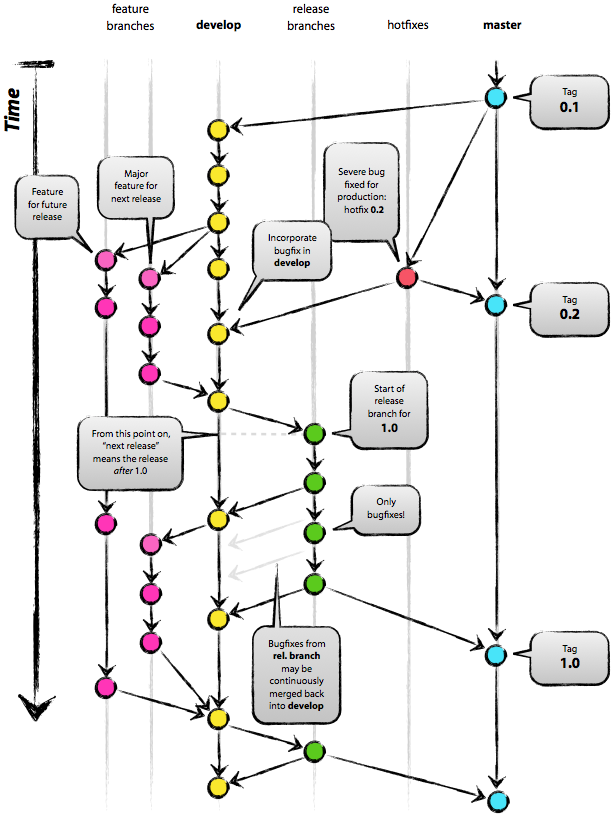
\includegraphics[scale=0.24]{n10.png}
    \end{column}
  \end{columns}
\end{frame}


